\chapter{Geometry of AdS$_{D+1}$}
\section{Global patch}
The global patch of AdS$_{D+1}$ is parametrised by the coordinates $(\rho,t, \Omega_D)$ where $\rho \in [0,\pi/2)$ is the radial coordinate (with the radial distance given by $\cos \rho$), $t \in (-\infty,\infty)$ is the time coordinate and $\Omega_{D-1}$ are the standard coordinates on the (D-1) dimensional sphere $S_{D-1}$. 

\begin{align}
 ds^2 = \frac{R^2}{\cos^2 \rho} \left( -dt^2 + d\rho^2 + \sin^2\rho d\Omega_{D-1}^2 \right) \label{globads}
\end{align}

\section{Poincar\'{e} patch}
The Poincar\'{e} patch of AdS$_{D+1}$ is parametrised by the coordinates $(u,x^0, x^1, \cdots x^D)$ (for $u \geq 0$, the upper half plane or UHP for short) where $u=0$ corresponds to the (conformal) boundary, and the metric is given by  

\begin{align}
 ds^2 = \frac{R^2}{u^2} \left( -dx_0^2 + du^2 + \sum_{i=1}^D dx_i^2 \right) \label{poincareads}
\end{align}


\section{Embedding Formalism}
Many calculations in AdS space are simplified by embedding AdS$_{D+1}$ in the D+2 flat space with metric
\begin{align}
 ds^2 = -dX_0^2 -dX_{D+1}^2+\sum_{i=1}^D dX_i^2
\end{align}
The AdS$_{D+1}$ space is then (the open cover of) the D+1 dimensional subspace defined by the equation
\begin{align}
 -X_0^2 -X_{D+1}^2+\sum_{i=1}^D X_i^2 = -R^2
\end{align}
or to be concise,
\begin{align}
 X^A X_A = -R^2 \label{embedads}
\end{align}


\section{Embedding Formalism(Euclidean)}
Many calculations in AdS space are simplified by embedding euclidean AdS$_{D+1}$ in the D+2 dimensional minkowski
\begin{align}
 ds^2 = -(dX^{-1})^2 +(dX^{0})^2+\sum_{i=1}^D (dX^i)^2
\end{align}

or introducing the light-cone coordinates $X^\pm = X^{-1} \pm X^0$,

\begin{align}
 ds^2 = -dX^+dX^-+\sum_{i=1}^D (dX^i)^2
\end{align}

The AdS$_{D+1}$ space is then (the open cover of) the D+1 dimensional subspace defined by the equation
\begin{align}
 -(X^{-1})^2 +(X^0)^2+\sum_{i=1}^D (X^i)^2 = -R^2
\end{align}
or to be concise,
\begin{align}
 X^A X_A = -R^2 \label{embedads}
\end{align}

The Poincar\'{e} coordinates on Euclidean AdS are then defined as 
\begin{align}
 X^+ = \frac{u^2 + |x|^2}{u}, \;\;\; Y^- = \frac{1}{u}, \;\;\; Y^i = \frac{x^i}{u}
\end{align}


In the embedding space, the infinitesimal generators of the group of Lorentz transformations in D+2 dimensions, SO(D+1,1) are 
\begin{align}
 L_{AB} = X_A \partial_B - X_B \partial_A
\end{align}
Moreover, the isometry group of euclidean AdS$_{D+1}$ is exactly SO(D+1,1), and so we can identify the generators $L_{AB}$ with the isometry generators of euclidean AdS$_{D+1}$
Then $L$ is a Casimir operator (an operator which commutes with all other operators in the algebra $[L,L_{AB}]=0$) with
\begin{align}
 L=\frac{1}{2} L_{AB}L^{AB} = \frac{1}{2}\left(X_A \partial_B - X_B \partial_A\right)\left(X^A \partial^B - X^B \partial^A\right)
\end{align}



Note that unlike Lorentzian AdS, in Euclidean AdS, the Poincar\'{e} coordinates cover the whole space, just like the global coordinates.

\section{Geodesics} \label{adsgeodesic}
One could calculate the geodesics in AdS$_{D+1}$ directly by extremising the following action
\begin{align}
 S= \int \mathrm{d} \lambda \; \sqrt{g_{\mu \nu} {\frac{dx^\mu}{d\lambda}} {\frac{dx^\nu}{d\lambda}} }
\end{align}
where for AdS$_{D+1}$ the metric $g_{\mu\nu}$ can be read off from \ref{globads} in global coordinates and \ref{poincareads} in Poincar\'{e} coordinates for the Poincare patch.

However, in practice this method gets fairly tedious and messy. Instead, it is customary to go to the embedding D+2 dimensional space and find the geodesics there subject to the contraint of equation \ref{embedads}. We shall work with the action [$(\cdot)^\prime = d(\cdot)/d\tau$]

\begin{align}
 S = \int {X^\prime}^A X^\prime_A + \lambda (X^A X_A + R^2 )
\end{align}

Where $\lambda$ is the lagrange multiplier. This gives the equations of motion
\begin{align}
 X_B^{\prime\prime} &= \lambda X_B \; \;\; B \in \{0,1,\cdots D+1 \} \\
 X^A X_A &= -R^2 
\end{align}
Let's focus on the first equation for now. Since the proper time $\tau$ is an unphysical coordinate and $\lambda$ is an arbitrary parameter, we can rescale $\tau \to \tau/\sqrt{|\lambda|}$. This gives for the first equation of motion:
\begin{align}
 X_B^{\prime\prime} = \frac{\lambda}{|\lambda|} X_B 
\end{align}
that is essentially we have 3 choices $\frac{\lambda}{|\lambda|} = -1, 0, 1$ and these exactly correspond to timelike, null and spacelike geodesics.

In particular, in Euclidean AdS$_3$ geodesics are semi-circles starting and ending on the boundary. Euclidean AdS$_3$ may be parametrised with the Poincar\'{e} coordinates $(u,x,y)$ with the metric
\begin{align}
 ds^2 = \frac{du^2 + dx^2 + dy^2}{u^2} 
\end{align}

The geodesic between two points on the boundary $(x_1,y_1)$ and $(x_2,y_2)$ may be parametrised with the coordinate $u$ and the length $\Delta l$ between two points may be written as 

\begin{align}
 \Delta l = \int \frac{du}{u} \sqrt{\dot{x}^2 + \dot{y}^2 +1}
\end{align}
where now $\dot x \equiv dx/du$. And so the geodesic equation can be derived using the Euler-Lagrange equations with $\mathcal{L} =  \sqrt{\dot{x}^2 + \dot{y}^2 +1}/{u}$. With some elementary algebra and integration, one ends up with the equation for a circle in the plane normal to the boundary $u=0$ and passing through the points $(x_1,y_1)$ and $(x_2,y_2)$. The semi-circular geodesic is uniquely defined by the fact that it meets the boundary $u=0$ perpendicularly. [Insert fig]



\subsection{Timelike geodesics}
The timelike geodesics are given by

\begin{align}
  X_B^{\prime\prime} = - X_B \label{timelike}
\end{align}
Subject to the constraint $ X^A X_A = -R^2$.
The eqn \ref{timelike} has the general solution:
\begin{align}
 X_B = c_B \cos\tau + d_B \sin \tau
\end{align}
Where $c_B, d_B$ are constant (no explicit $\tau$ dependence) vectors subject to constraints due to $ X^A X_A = -R^2$ :
\begin{align}
 &c_A d^A = 0 \\
 &c_A c^A = -R^2 = d_A d^A 
\end{align}

A common approach is to parametrise the timelike (massive) geodesic in AdS with the global coordinates $(\rho, t, \Omega_{D-1})$. Identify $\tau \equiv t$, and then parametrise $c_A, d_A$ in terms of $\rho, \Omega_{D-1}$. The simplest solution is limiting to constant $\Omega_{D-1}$, choose 
\begin{align}
 &c^0=R=d^{D+1} \\
 &c^A=0=d^B \;:otherwise
\end{align}
This gives
\begin{align}
 &X^0 = R\cos t \\
 &X^{D+1} = R \sin t \\
 &X^A = 0 \; :otherwise
\end{align}

%\begin{figure}
 \centering
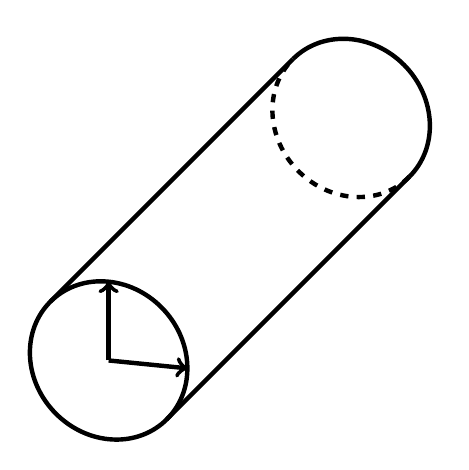
\begin{tikzpicture}

\begin{scope}[x={(1cm,-.1cm)}]
\path (1,0,0);
\pgfgetlastxy{\cylxx}{\cylxy}
\path (0,1,0);
\pgfgetlastxy{\cylyx}{\cylyy}
\path (0,0,1);
\pgfgetlastxy{\cylzx}{\cylzy}
\pgfmathsetmacro{\cylt}{(\cylzy * \cylyx - \cylzx * \cylyy)/ (\cylzy * \cylxx - \cylzx * \cylxy)}
\pgfmathsetmacro{\ang}{atan(\cylt)}
\pgfmathsetmacro{\ct}{1/sqrt(1 + (\cylt)^2)}
\pgfmathsetmacro{\st}{\cylt * \ct}
%\fill[red] (\ct,\st,0) -- ++(0,0,-8) arc[start angle=\ang,delta angle=180,radius=1] -- ++(0,0,8) arc[start angle=\ang+180,delta angle=-180,radius=1];
\begin{scope}[every path/.style={ultra thick}]
\draw (0,0,0) circle[radius=1];
\draw[->] (0,0,0) -- (1,0,0);
\draw[->] (0,0,0) -- (0,1,0);
\draw (\ct,\st,0) -- ++(0,0,-8);
\draw (-\ct,-\st,0) -- ++(0,0,-8);
\draw (\ct,\st,-8) arc[start angle=\ang,delta angle=180,radius=1];
\draw[dashed] (\ct,\st,-8) arc[start angle=\ang,delta angle=-180,radius=1];
\end{scope}
\end{scope}
\end{tikzpicture}
\end{figure}

\subsection{Null geodesics}
The null geodesic equation $ X_B^{\prime\prime} = 0$ has the general solution
\begin{align}
 X_B = c_B \tau + d_B
\end{align}
Along with the constrain equation $X^A X_A = -R^2$ this gives
\begin{align}
 &c_Ac^A = 0 = c_Ad^A \\
 &d_Ad^A=-R^2
\end{align}

